\documentclass[a4paper,11pt]{article}
\usepackage[francais]{babel}
\usepackage{amssymb}
\usepackage{graphicx}
\usepackage{listings}
\usepackage[hidelinks]{hyperref}
\usepackage[utf8]{inputenc}
\usepackage[T1]{fontenc}

\usepackage{graphicx}
\usepackage{float}


\hypersetup{
	colorlinks = true,
	linkcolor = red,
	urlcolor = blue,
	filecolor = blue
}

\author{Boris Berger\\Daniele Siragusa\\Giorgi Shavgulidze\\Thomas Perez}
\title{Développement d'Application Réticulaire\\Rapport\\PariServices}

\begin{document}

\maketitle
\newpage

\tableofcontents
\newpage

\section{Introduction}
PariServices est une application web offrant à ses utilisateurs la possibilité de demander et/où de rendre des services sur Paris. L'application permet entre autre à ses utilisateurs de localiser via l'API Google Maps le lieux auquel le service devra être rendu. Elle offre par ailleurs tout un système de gestion des comptes utilisateurs, qui permet à chaque memebre de savoir ses services demandé et offerts en cours.
\newline
L'application a pour finalité de pallier à deux manques de la société actuelle que sont le manque de temps et le manque d'argent. L'idée est de permettre à la première catégorie de déléguer certaines de ses tâches, moyennant finance, et d'offrire à la seconde catégorie une source de revenu. L'application est donc fortement orientée communauté.

\section{Manuel utilisateur}
Dans cette partie on vous expliquera comment profiter de site PariService en décrivant le manuel d'utilisation des fonctionnalités proposés. 
\subsection{L'obtention d'un profil}
Pour utiliser les services proposées par le site PariServices, vous allez besoin d'une compte utilisateur et pour l'obtenir on appuie sur le bouton \textbf{Créer un compte} et on remplit la formulaire comme ci-dessous.\newline

\begin{minipage}{0.53\textwidth}
	\begin{figure}[H]
		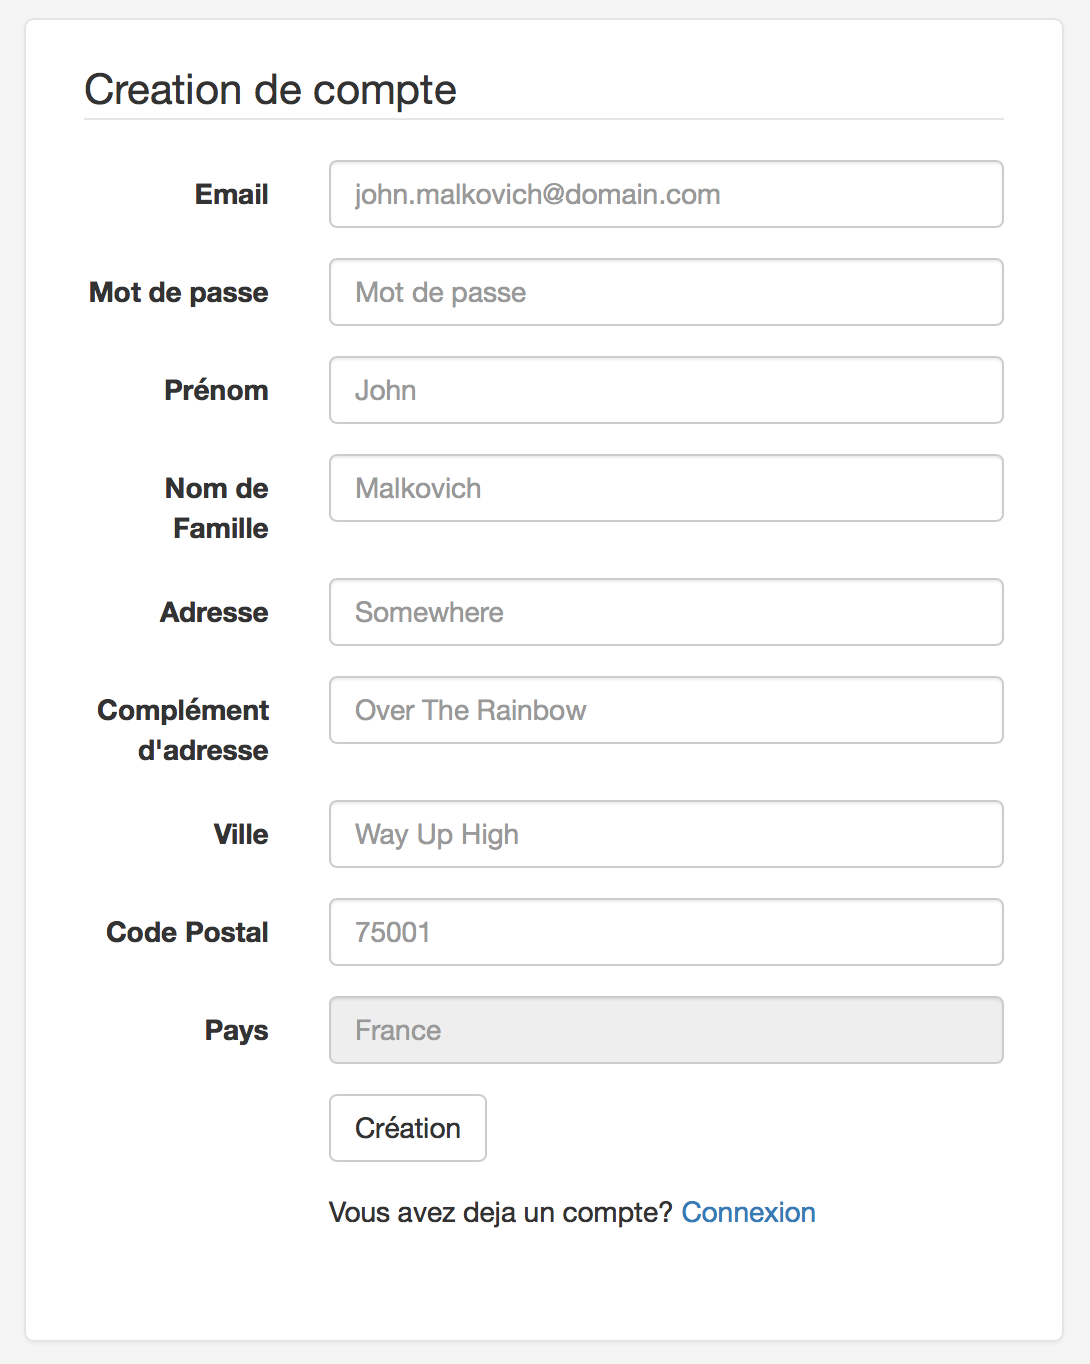
\includegraphics[width=1\textwidth]{images/manuel/signup}
		\caption{Page d'inscription \label{overflow}}
	\end{figure}
\end{minipage} \hfill
\begin{minipage}{0.45\textwidth}
\subparagraph{Inscription.}Après avoir rempli la forme correctement avec un bouton \textbf{Création} on sera redirigé sur la page principale de \textbf{\textit{PariServices}}, sinon les erreurs correspondants seront affichés.\newline
\subparagraph{Authentification.} Dans le cas où vous avez déjà un compte, vous pouvez l'accéder en entrant votre mail et mot de passe sur la page d'authentification.
\begin{figure}[H]
	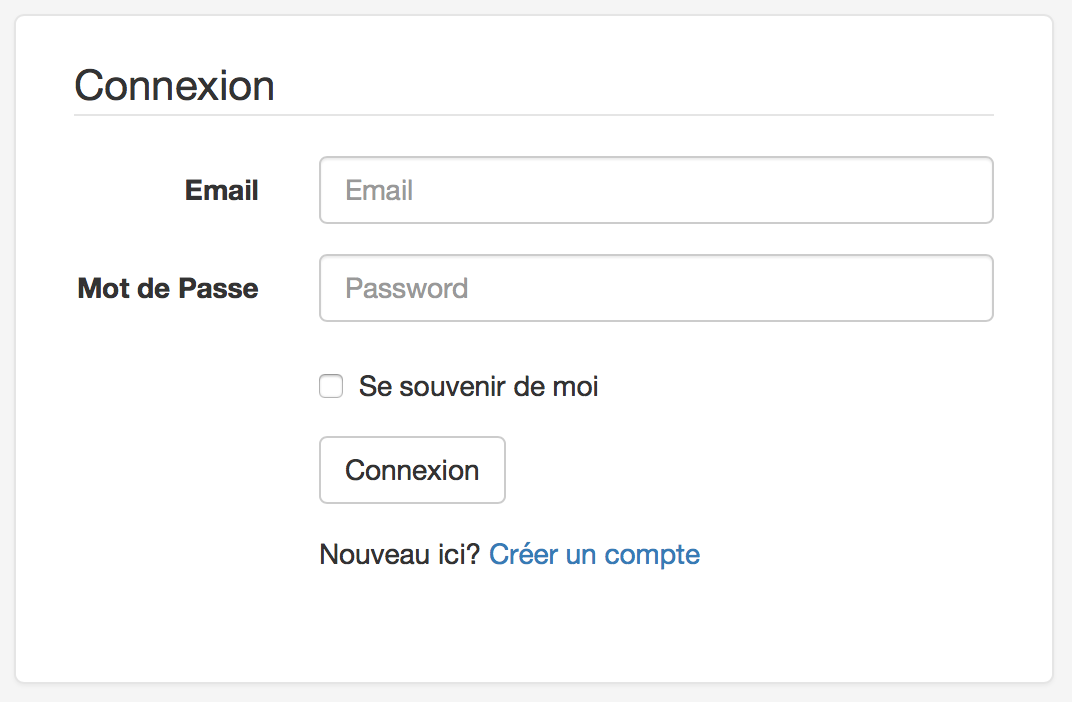
\includegraphics[width=1\textwidth]{images/manuel/signin}
	\caption{Authentification \label{overflow}}
\end{figure}
\end{minipage}\\\\\\

La page principale vous propose de choisir parmi les actions suivantes: \textbf{Rendre un service}, \textbf{Demander un service}, \textbf{Gestion de la profile} et \textbf{Déconnexion}.

\newpage
\subsection{La gestion d'un profil}
La page de profile d'utilisateur nous propose 5 onglets différents:

\subparagraph{Informations} visualise nos informations personnelles.

\begin{figure}[H]
	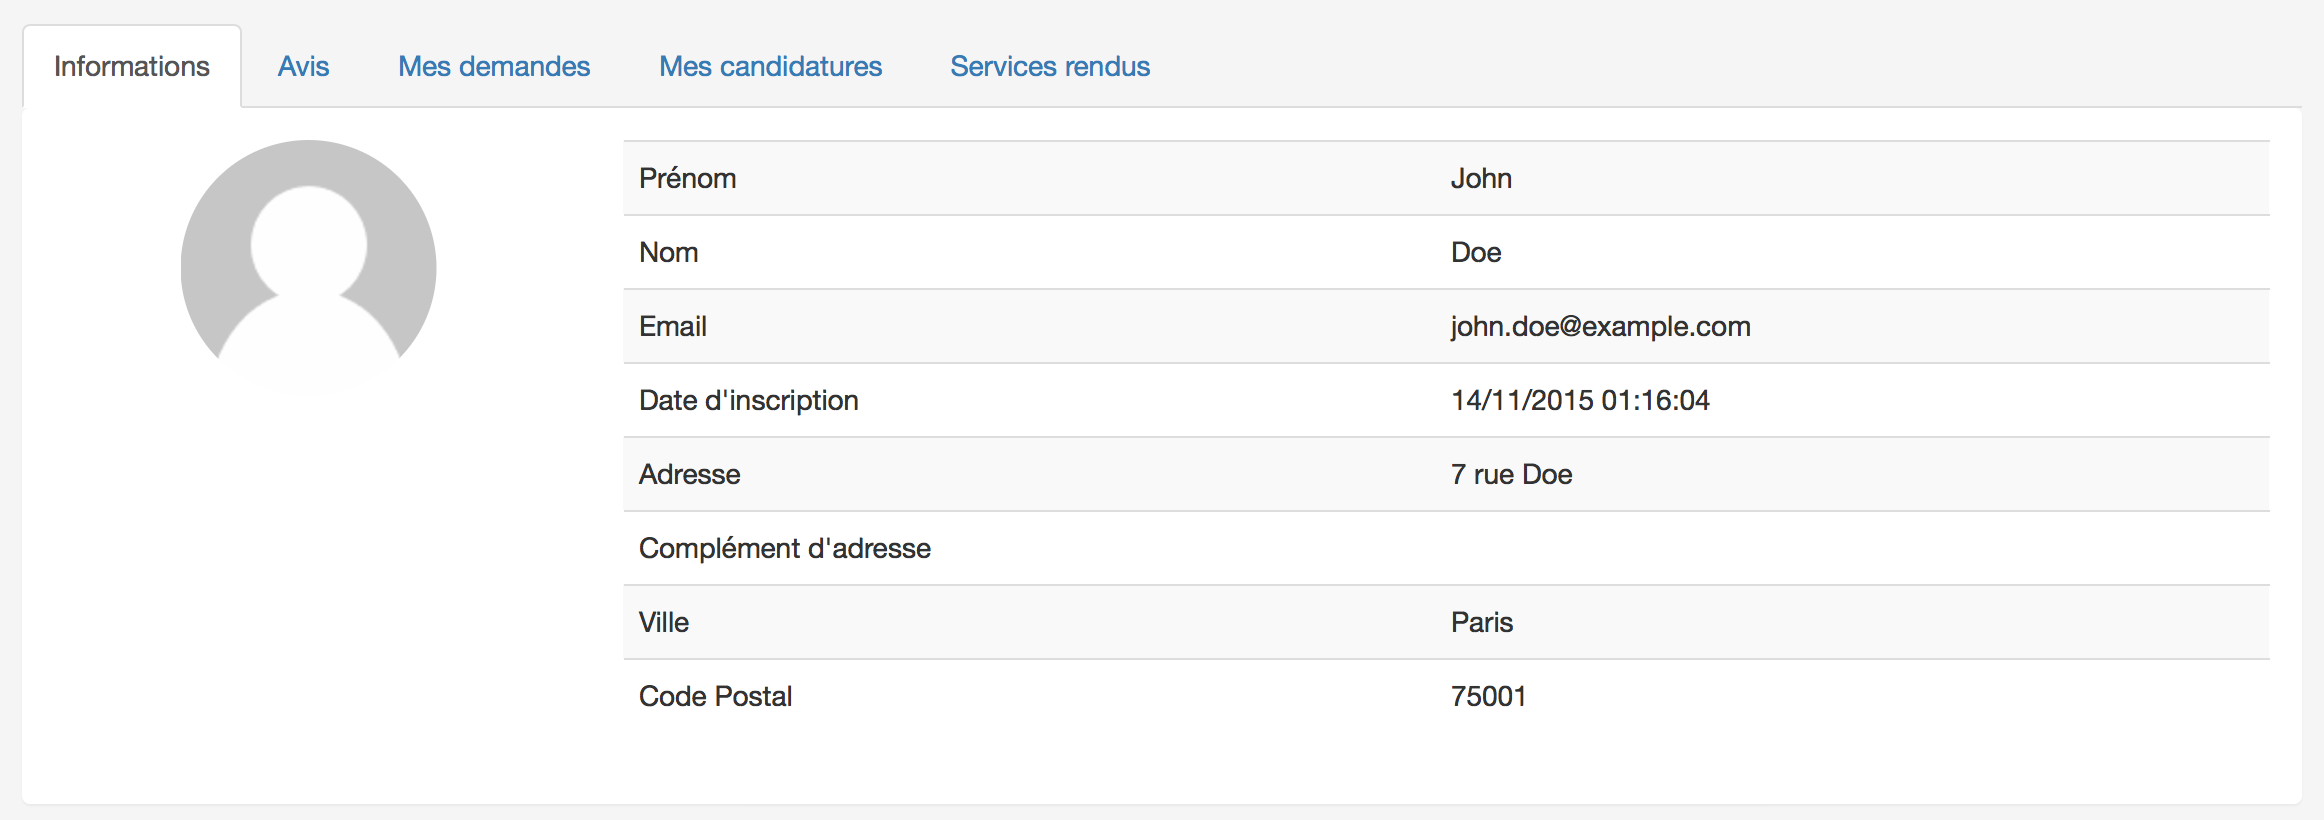
\includegraphics[width=1\textwidth]{images/manuel/profile}
	\caption{Page de la profile \label{overflow}}
\end{figure}

\subparagraph{Avis:} Les évaluations laissés par d'autre utilisateurs qui ont déjà rendu des services pour vous ou pour qui vous avez rendu des services.

\subparagraph{Mes demandes} affiche la liste des services qu'on a annoncé.

\subparagraph{Mes candidatures} affiche la liste des services sur lesquels on a présenté  notre candidature.
\subparagraph{Services rendus} affiche la liste des services qui sont déjà terminé et dans lesquels on a participé soi comme demandeur soit comme candidat.

\subsection{Demander un service}
\begin{minipage}{0.50\textwidth}
	Voici la forme à remplir pour demander un service. Essayer de bien remplir cette forme pour que gens puisse s'intéresser de votre annonce . Aussi c'est très important de correctement spécifier la catégorie et des tags car cela permet aux utilisateurs filtrer et chercher des annonces qui peuvent les intéresser. Après la date spécifié dans \textbf{Fin des candidatures} votre annonce sera automatiquement terminé et plus visible pour d'autres utilisateurs.
	\indent\paragraph{} Appuyer  sur \textbf{Submit} pour placer votre demande sur PariServices.
\end{minipage} \hfill
\begin{minipage}{0.45\textwidth}
	\begin{figure}[H]
		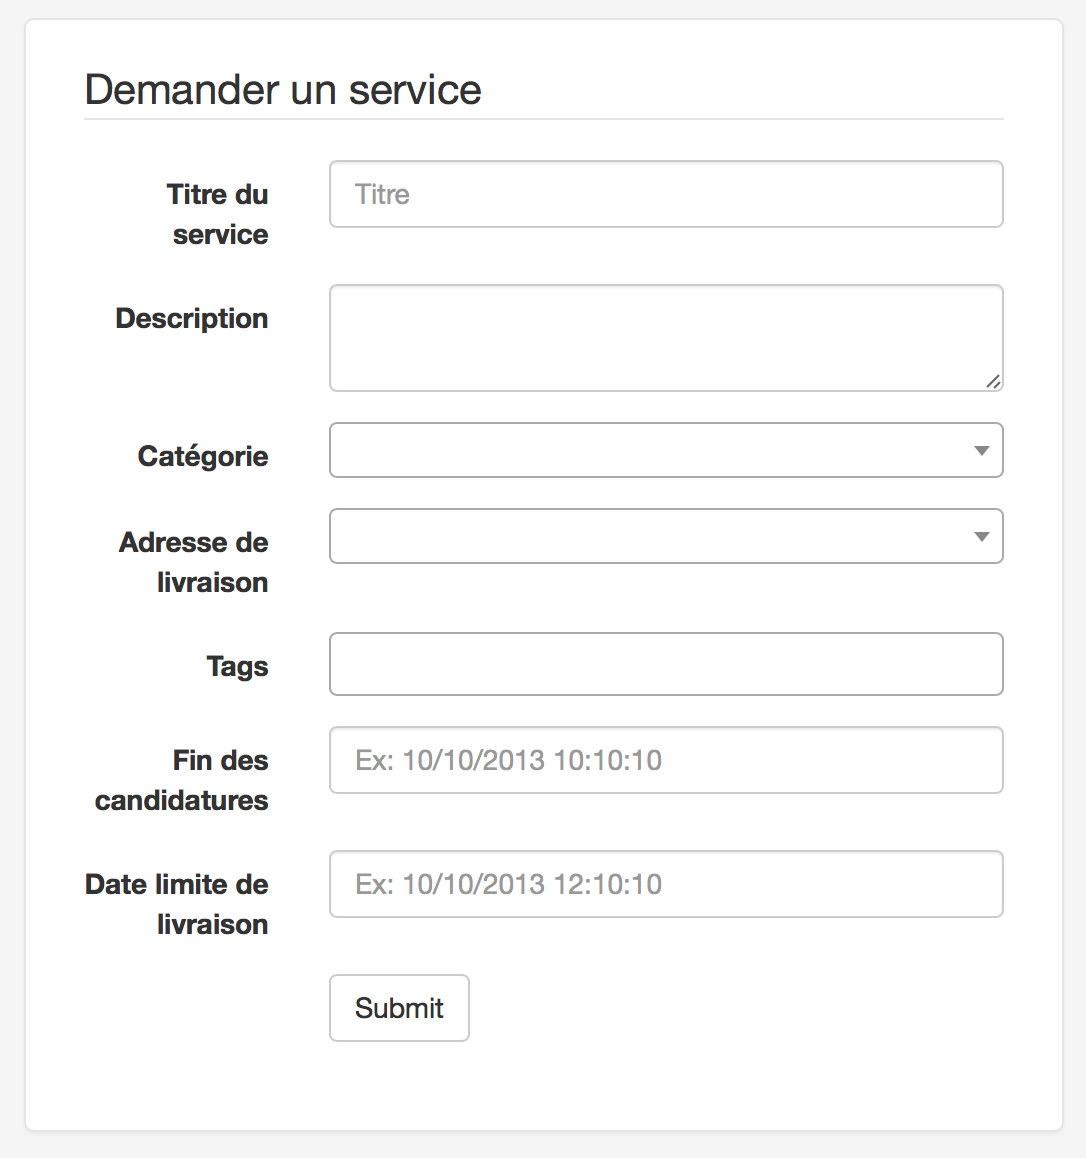
\includegraphics[width=1\textwidth]{images/manuel/demander}
		\caption{Page d'inscription }
	\end{figure}
\end{minipage}\\\\\\


\subsection{Rendre un service}
La page de \textbf{Rendre un service} contient bar de recherche (\textit{Figure ~\ref{fig:recherche}}) et la liste des résultats correspondant à les critères de recherche. Sur la \textit{Figure ~\ref{fig:resultat}} on voie une exemple de recherche avec un tag "New tag" et la liste des résultats contient une annonce nommée "New Example". 

\begin{figure}[H]
	
\includegraphics[width=1\textwidth]{images/manuel/recherche}
	\caption{Bar de recherche }
	\label{fig:recherche}
\end{figure}
\begin{figure}[H]
	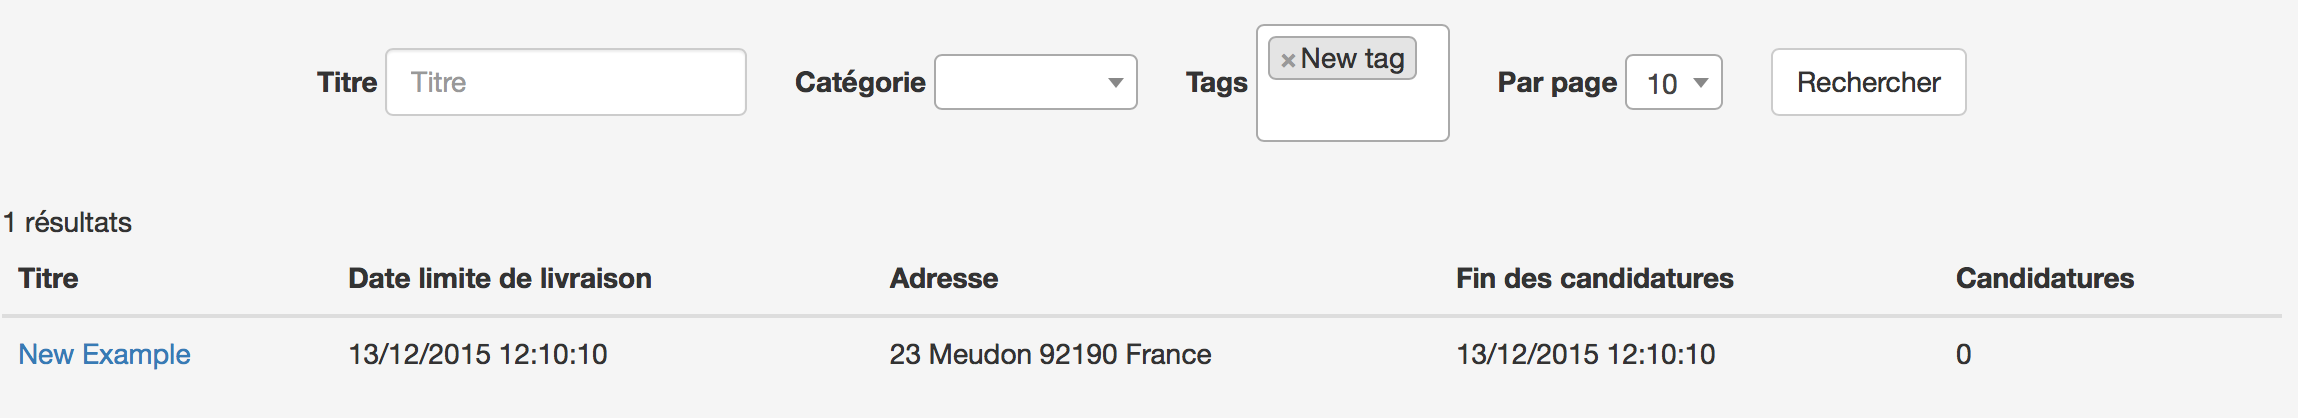
\includegraphics[width=1\textwidth]{images/manuel/resultat}
	\caption{Résultats de recherche }
	\label{fig:resultat}
\end{figure}

\paragraph{}
En appuyant sur le nom de demande on peut visualiser l'annonce qui contient 3 parties principales: 
\begin{enumerate}
	\item Informations sur (\textit{Figure ~\ref{fig:infoannonce}})
	\begin{itemize}
		\item demandeur
		\item description de l'annonce
		\item adresse de rendez-vous
	\end{itemize}
	\item La forme à remplir pour visualiser le chemin optimal de notre adresse vers l'adresse de rendez-vous.  (\textit{Figure ~\ref{fig:formeadresse}})
	\item La carte Google Maps
\end{enumerate}

\begin{figure}[H]
	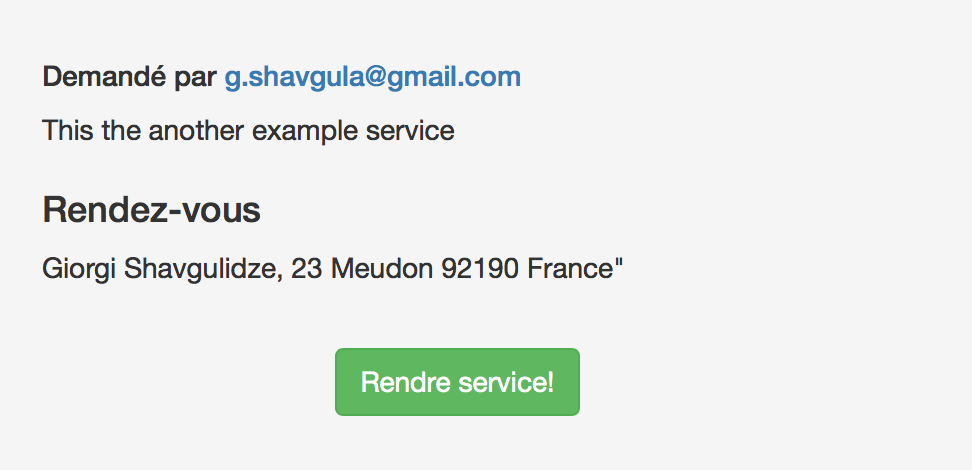
\includegraphics[width=1\textwidth]{images/manuel/demandeur}
	\caption{Informations sur demandeur \& annonce }
	\label{fig:infoannonce}
\end{figure}
\begin{figure}[H]
	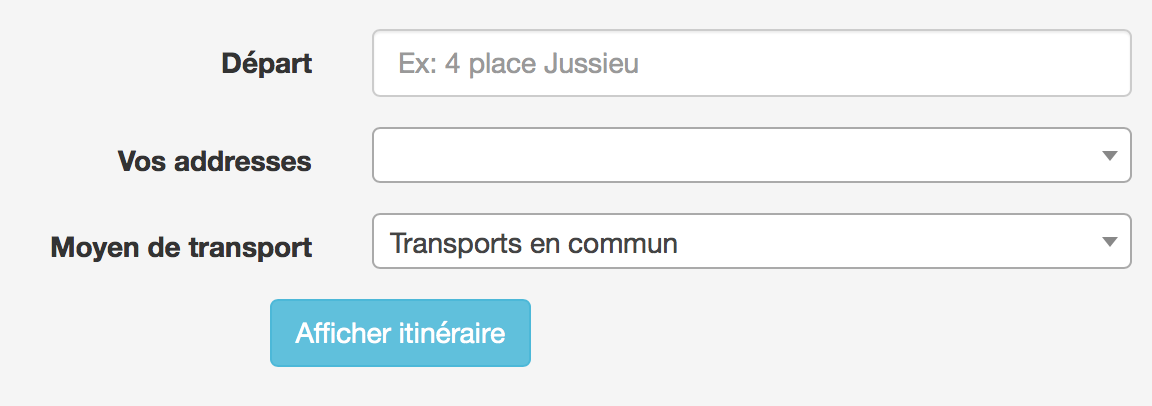
\includegraphics[width=1\textwidth]{images/manuel/adresse}
	\caption{Comment y arriver? \label{overflow}}
	\label{fig:formeadresse}
\end{figure}

\pagebreak

\subsection{Interface}
Ici sera la description de l'interface...
\subsection{Case d'utilisation}
Ici sera la description des cas d'utilisation...


\section{Développement}
Ici sera le développement...

\subsection{Schéma de l'application}
Ici sera le schéma de l'application...

% ne pas seulement parler des choix technologiques
\subsection{Choix techniques}
Ici sera la description de nos choix techniques...

% courte description des tehcnologies, surtout justifier leur utilisation
\subsection{Technologies}
Ici sera la description des technologies utilisées...



\section{Fonctionnalités}
Ici sera la description des fonctionnalités...
\subsection{Points forts}
Ici sera la description des points forts de notre application...
\subsection{Points faibles}
Ici sera la description des points faibles de notre application...
\subsection{Non implémentées}
Ici sera la description des fonctionnalités non implémentées...



\section{Compléments}

\subsection{Extensions possibles}

\subsubsection{Système de notifications}
Pour l'heure, les volontaires sont notifiés via l'envoie d'un mail lorsqu'ils sont sélectionnés pour une tâche. L'idée serait de se changer ce système pour des notifications internes au site. Ces notifications seraient signalées à l'utilisateur via un petit popup aparaissant dans le header de la page, près du lien vers le profil de l'utilisateur. Lors de l'arrivée sur son profil, l'utilisateur serait alors informé de son acceptation via un message plus explicite.

\subsubsection{Système d'administration}
On imagine bien qu'une application permettant aux utilisateurs de demander des services contre de l'argent pourrait facilement être utilisée à des fins illégales. Pour prévenir ce genre d'abus, plusieurs solutions nous semble possible:

\begin{itemize}
\item la mise en place d'administrateurs chargés de valider et de supprimer les annonces dites "illégales". Cela supposerait plusieurs ajouts, notamment une nouvelle table dans la base de donnée qui stockerait les administrateurs. De nouveaux boutons permettant de supprimer ou de modifier une annonce apparaîteraient alors lorsqu'un administrateur arriverait sur la page d'une annonce. Il faudrait également ajouter la possibilité de bannir un utilisateur, avec l'ajout d'un bouton accessibles uniquement aux administrateurs sur la page de profil d'un utilisateur. Une dernière idée serait d'ajouter sur la page des services un bouton "Signaler l'annonce". Visible par tous, ce boton permettrait d'envoyer une notification aux  administrateurs du site qui leur permettrait de venir contrôlé l'annonce.
\item l'implantation d'une tâche automatisée chargée de parcourire les annonces dus site à interval régulier et de supprimer automatiquement les annonces. La tâche pourrait par exemple parser les champ des annonces à la recherche de mots révélateurs. Cette solution poserait de nombreux problèmes de concurrence, notament avec notre tâche ettant à jour les annonces ayant dépassé leur date de rendu.
\end{itemize}

\subsubsection{Calcul du temps nécessaire à la satisfaction d'un service}
L'API Google Maps permet de connaître la distance séparant deux points sur la carte. Nous pourrions utiliser cette information qui, couplée au moyen de transport, pourrait nous permettre d'offrire à l'utilisateur une estimation du temps qu'il mettra à accomplir le service. Nous pourrions alors, en comparant à la date courante de l'utilisateur, signaler à l'utilisateur qu'il ne pourra pas accomplir ce service dans les temps.

\subsubsection{Intégration d'un système de paiement}
Actuellement, le paiement des services est laissé à la discrétion des utilisateurs. Nous pourrions intégrer la mécanique de paiement directement au site via un service comme paypal par exemple. Il faudrait alors notament se poser la question de la politique de paiement. Le volontaire pourrais par exemple être payer la moitié de la somme au moment ou il est sélectionner et l'autre moitié après confirmation du client que le service a bien été rendu.

\subsubsection{Intégration d'un système de réputation}
Permettre aux utilisateurs de s'évaluer entre eux au fil des transactions leur permettrait de mieux sélectionner leurs intermédiaires. On pourrait imaginer que le système de réputation soit diviser en deux: en tant que volontaire et en tant que demandeur. La réputation prendrait la forme d'un score global avec des évaluations au format texte.

\subsubsection{Respect de la norme ARIA}
De part son concept, notre application s'adresse tout particulièrement aux personnes ne pouvant pas sortir de chez elles du fait d'un handicap. Or, la norme ARIA offre un ensemble de propriétés qui, si elles sont respectées, garantissent l'accessibilité du site pour les personnes handicapées. Le non-respect de cette norme nous couperais donc l'accès à une énorme partie de notre publique potentiel. L'application de la norme n'est néanmoins pas immédiat et son respect impliquerais de nombreuses modifications dans l'interface de notre site.

\subsection{Monétisation}
La monétisation de notre application découle directement de notre amélioration intégrant le système de paiement à notre site. L'idée serait alors de prélever un pourcentage sur chaque transaction effectuée. Une autre idée serait d'offrire des services supplémentaires payant. Par exemple l'ajout de photos supplémentaires pour les annonces ou un système permettant aux utilisateurs de programmer automatiquement l'ajout d'annonce de façon périodique.


\section{Conclusion}
Notre application nous a permis de manipuler de nombreuses technologies que jusque là aucun membre du groupe n'avait utiliser. Nous avons pu constater la puissance des technologie Spring et Hbernate qui, combinées, offrent une élégance ainsi qu'un puissant contrôle pour le développement de l'application. Nous avons par ailleurs apprécier de découvrire ces technologies particulièrements populaire dans le monde de l'entreprise. Le groupe a également acquis une meilleure vision d'ensemble de c qu'est le développement d'une application web à l'échelle commerciale.

\end{document}
